\documentclass{report}
\usepackage[T2A,T1]{fontenc} % Add this line for Cyrillic support
\usepackage{fontspec} % Add this line
\setmainfont{Times New Roman}
\usepackage{lipsum}
\usepackage{gensymb}
\usepackage{float}
\usepackage{graphicx} % Required for inserting images

\usepackage{cite}
\usepackage{caption}

\usepackage{tabularx}
\usepackage{booktabs}
\usepackage{longtable}
\usepackage{pdflscape}

\usepackage{graphicx}
\usepackage{svg}
\usepackage{xcolor}
\usepackage{tikz}
\usepackage{hyperref}
\usepackage{multirow}
\usepackage{enumerate}
\usepackage[shortlabels]{enumitem}
\usepackage{amsmath}
\usepackage{nomencl} % For nomenclature and acronyms
\selectlanguage{english}
\makenomenclature % Activate nomenclature

\definecolor{lightblue}{HTML}{a0d8ef}

\title{Research Report - 5G Security Analysis} %title of the file

\begin{document}
\selectlanguage{english}
%----------- Report information ---------

\logo{logos/ULB_round.png}
\uni{\textbf{Université Libre de Bruxelles}}
\ttitle{5G Security Analysis - Security of Critical Interfaces and Zero Trust Architecture} %title of the file
\subject{Mobile and Wireless Networks} % Subject name
\topic{Research Report} % Topic name

\professor{Prof. \textsc{Dricot} Jean-Michel} % information related to the professor

\students{  \textsc{Ali-Khodja} Myriam Erin Johanna\\
            \textsc{Hassani} Mortaza\\
            \textsc{Amanor} Deborah\\
            \textsc{Bouta} Ali} % information related to the students

%----------- Init -------------------

\buildmargins % display margins
\buildcover % create the front cover of the document
\toc % creates the table of contents

%------------ Report body ----------------

\section*{Abstract}
Zero Trust Architecture (ZTA) has been implemented in 5G networks to enhance security between fragmented components, such as the NG-RAN and 5GC. However, its application to securing 5G critical interfaces and the broader 5G architecture remains underexplored. 5G networks face significant security challenges, particularly at critical interfaces like N1, N2, N3, and SBIs, which handle sensitive data and interconnect network functions. This report analyzes vulnerabilities in these interfaces, evaluates ZTA’s potential for enhancing their security, and highlights gaps in existing literature. The findings provide valuable insights into leveraging ZTA for a unified and resilient security framework across 5G systems.

\section{Introduction}
The transition to 5G networks presents significant security challenges due to their highly dynamic, distributed, and virtualized architecture. Traditional perimeter-based security models are no longer sufficient, as the complexity and interconnectedness of the network expose new vulnerabilities. One promising solution to these challenges is the adoption of Zero Trust (ZT) security architecture, which assumes no implicit trust within the network and enforces strict verification of all entities, regardless of their origin. This approach is well-suited for the 5G environment, where constant authentication, granular access control, and the principle of least privilege are essential for maintaining security.

In parallel, critical interfaces within the 5G architecture play a central role in connecting the various network functions. These interfaces—such as N1, N2, N3, and Service-Based Interfaces (SBIs)—enable communication between different components across OpenRAN, vRAN, and CloudRAN deployments. However, their pivotal role in data exchange and signaling also makes them potential targets for cyberattacks. As these interfaces connect a wide range of network functions, securing them is paramount.

This report aims to assess the current state of Zero Trust implementation in 5G networks and analyze the security principles applied to critical interfaces. By evaluating existing security measures, identifying vulnerabilities, and examining best practices recommended by standardization bodies, this work will provide insights into strengthening the security of 5G interfaces and the overall network infrastructure.

\subsection{Problem Statement}
Security analyses of 5G networks often lack a targeted focus on the critical interfaces that connect the NG-RAN and the 5G core network to external entities. Although Zero Trust Architecture has been applied to the network functions within the 5G core and RAN, its implementation across the entire 5G system architecture remains fragmented. This limitation leaves critical interfaces vulnerable to emerging threats. 


\subsubsection{Research goal}
This study aims to achieve the following objectives:
\begin{itemize}
    \item Conduct a comprehensive analysis of the threats and vulnerabilities associated with 5G critical interfaces, including N1, N2, N3, and SBIs.
    \item Explore the application of Zero Trust Architecture across the entire 5G system to.
    \item Identify security gaps and propose enhanced security measures to strengthen the protection of critical interfaces using ZTA.
\end{itemize}

\subsection{Methodology}
To achieve the goal of this research, we conducted a comprehensive literature  to analyze existing studies on 5G critical interface security and the application of Zero Trust Architecture (ZTA). Research questions were formulated to guide the study which will be discussed in detail in subsequent sections. 


\section{Background}
\textbf{\textit{The evolution of 5G}}\\
The fifth generation of mobile networks, represents a revolutionary leap compared to its predecessors (2G, 3G, and 4G). While earlier generations primarily focused on improving voice communication, data speeds, and internet access, 5G goes much further by enabling entirely new applications and use cases. With speeds up to 100 times faster than 4G and latencies as low as 1 millisecond, 5G introduces the capacity to support massive device connectivity and mission-critical, real-time applications.\\Unlike previous networks, 5G is designed to seamlessly integrate with emerging technologies such as autonomous vehicles, augmented reality (AR), industrial automation, and the Internet of Things (IoT). Its architecture supports network slicing, which allows operators to create virtualized networks tailored to specific applications or industries. These capabilities make 5G a cornerstone for the digital transformation of industries and services.

\begin{figure}[h]
    \centering
    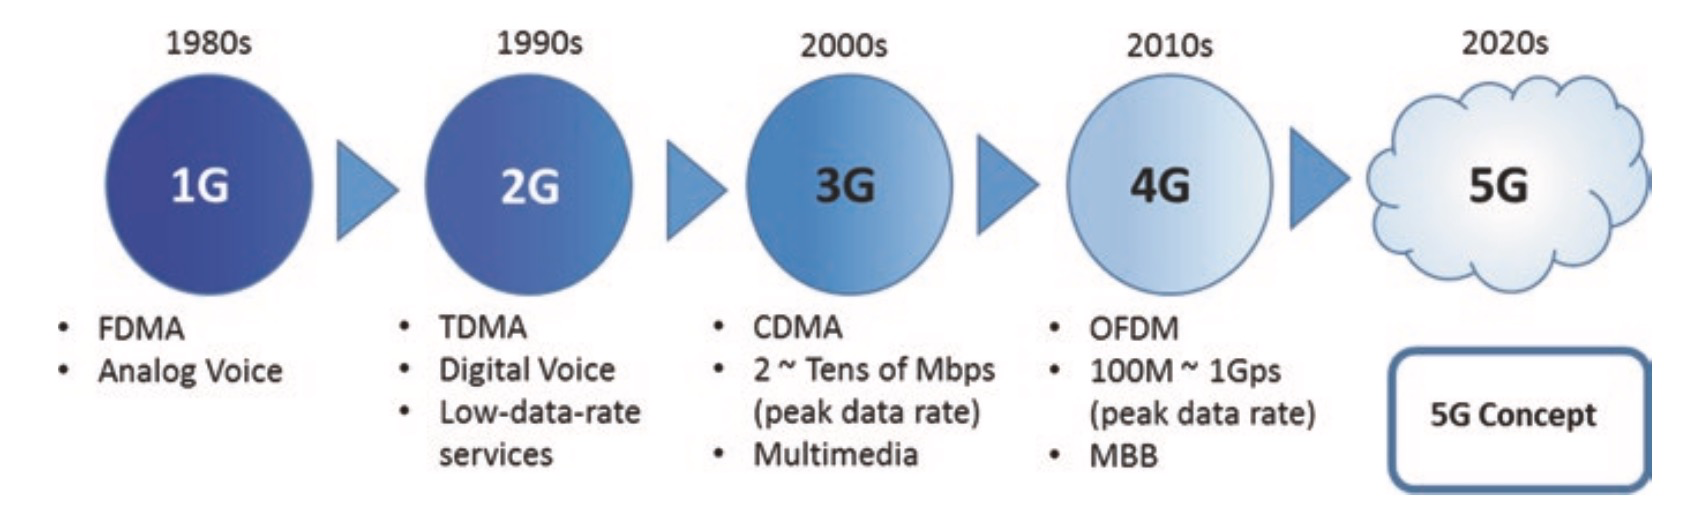
\includegraphics[width=0.85\textwidth]{figures/1gto5g.png}
    \caption{Cellular network evolution by generation\cite{wan_lei_2020}}
    \label{fig:history1gto5g}
\end{figure}

\textbf{\textit{Security Challenges in 5G Networks}}\\
While 5G holds immense potential, it also brings new security challenges due to its highly distributed and software-driven architecture. Features such as virtualized network functions (VNFs), edge computing, and dense device connectivity expand the attack surface, increasing the risk of cyberattacks. Traditional security models that relied on perimeter-based defenses are no longer sufficient, as attackers can exploit vulnerabilities across interconnected systems and networks.\\\\

\textbf{\textit{The Need for Zero Trust}}\\
To address the security challenges posed by 5G networks, adopting a Zero Trust (ZT) security model is essential. Unlike traditional models that assume trust within the network perimeter, Zero Trust operates on the principle of "never trust, always verify," assuming that both internal and external threats are always present. This approach requires strict verification of all entities—whether users, devices, or applications—before granting access. It emphasizes continuous monitoring, dynamic policy enforcement, and granular access controls based on factors such as user identity, device posture, and other contextual elements. Zero Trust aligns perfectly with the dynamic and distributed nature of 5G, helping to mitigate risks like lateral movement and unauthorized access within a network. By reducing implicit trust, it ensures that all interactions are continuously verified, providing high levels of security without compromising the performance or scalability required by 5G networks.
\section{5G Architecture}
This section highlights the 5G components, the different deployment type and the protocols used.
\subsection{5G Components}
\begin{enumerate}
    \item \textbf{User Equipment (UE)}: Refers to devices such as smartphones, IoT devices, and wearables that connect to the 5G network. They interact with the network through radio access, enabling 5G services for users.
    \item \textbf{Core Network (CN)}: Manages data traffic, authentication, and service delivery across the 5G network. It connects access networks and handles functions like routing, security, and service management.
    \item \textbf{Radio Access Network (RAN)}: Facilitates wireless communication between User Equipment and the Core Network. Composed of base stations and antennas, it provides the radio signals necessary for 5G connectivity.
\end{enumerate}

\subsection{The evolution of RAN}
\textit{- Traditional RAN:} The traditional RAN, used from 2G to 5G, connects end users with remote-control systems via the core network and consists of base stations, baseband units (BBUs), and controllers; however, its proprietary technologies limit options for equipment and software.\\
\textit{- Centralized RAN (CRAN):} CRAN moves the baseband unit (BBU) from the individual base stations to a centralized location, allowing for more efficient use of resources, reduced costs, and better coordination of network traffic, but it requires high-bandwidth backhaul connections.\\
\textit{- Virtualized RAN (vRAN):} With the advancement of network function virtualization (NFV) and software-defined networks, vRAN replaces traditional hardware by virtualizing the baseband unit into separate distribution and control units, allowing for a more flexible, cloud-based architecture with centralized BBUs and software-based controllers, though it still relies on proprietary radios and interfaces.\\
\textit{- Disaggregated vRAN:} Disaggregated vRAN further evolves from traditional vRAN by separating hardware and software elements across different vendors, enabling greater flexibility and scalability; it allows baseband units to be virtualized and deployed across distributed locations, reducing reliance on a single vendor and fostering a more open ecosystem.\\
\textit{- Open RAN (ORAN):} Building upon vRAN, ORAN focuses on openness and standardization, promoting interoperability between vendors through open interfaces, and uses NFV and SDN to enable network slicing, providing a more flexible and scalable architecture, though it still faces challenges related to integration and multi-vendor compatibility.

\begin{figure}[h]
    \centering
    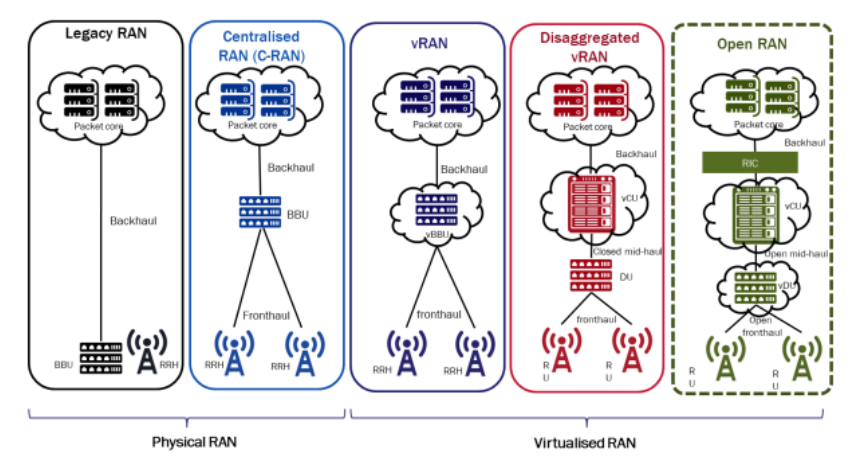
\includegraphics[width=0.79\linewidth]{figures/rantypes.png}
    \caption{Evolution of the RAN architecture\cite{moniem_vran_openran}}
    \label{fig:RANarchtypes}
\end{figure}

\subsection{5G Core Network}
The 5G Core Network (5GC) is the central component of the 5G architecture, responsible for managing data traffic, providing essential network functions, and enabling advanced capabilities such as network slicing and low-latency communication.
\begin{figure}[H]
    \centering
    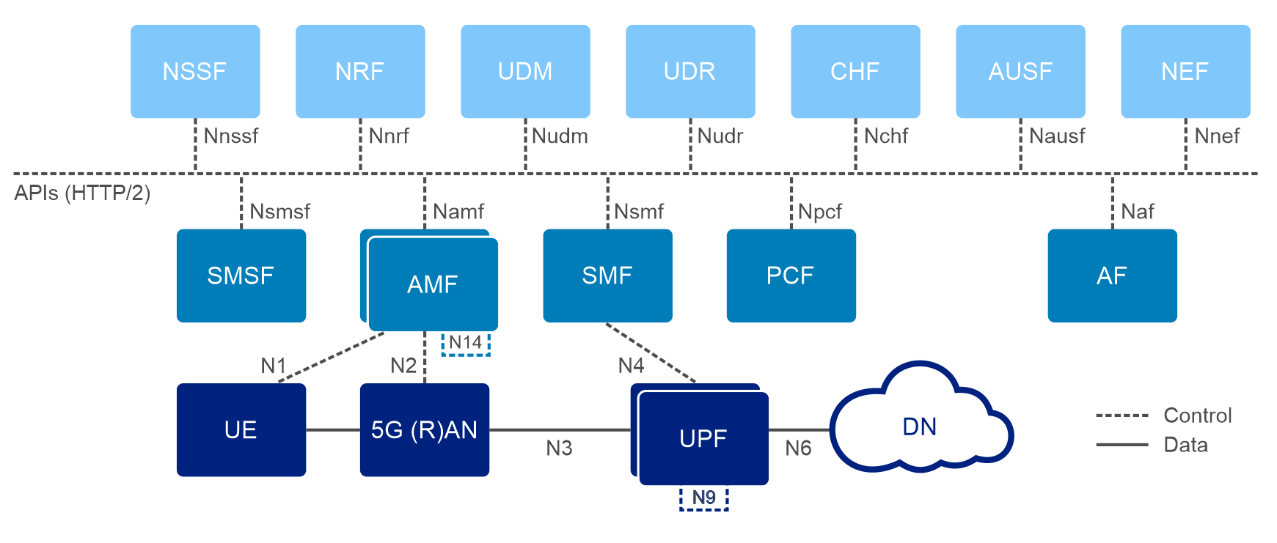
\includegraphics[width=0.8\linewidth]{figures/5GC.png}
    \caption{5GC Architecture \cite{dolente2023vulnerability}}
    \label{fig:5GCarch}
\end{figure}

\begin{table}[H]
    \centering
    \begin{tabularx}{\textwidth}{lX}
        \toprule
        \textbf{Function} & \textbf{Main Role} \\
        \midrule
        Access and Mobility Management Function (AMF) & Supervises network access, connection, and mobility. \\
        \addlinespace
        Session Management Function (SMF) & Manages network sessions, QoS parameters, routing, and billing information. \\
        \addlinespace
        Authentication Server Function (AUSF) & Facilitates the authentication of UE (User Equipment). \\
        \addlinespace
        Network Slice Selection Function (NSSF) & Selects network slice instances (NSI) based on UE performance requirements. \\
        \addlinespace
        Network Repository Function (NRF) & Manages the lifecycle of network function profiles. \\
        \addlinespace
        Policy Control Function (PCF) & Generates and applies network control policies. \\
        \addlinespace
        Network Exposure Function (NEF) & Exposes network functionalities securely to external applications. \\
        \addlinespace
        Unified Data Management (UDM) & Manages subscription-related information. \\
        \addlinespace
        Unified Data Repository (UDR) & Stores subscription information accessible by UDM. \\
        \addlinespace
        User Plane Function (UPF) & Manages the transmission of user data. \\
        \bottomrule
    \end{tabularx}
\end{table}

\subsection{The Critical 5G interfaces}
Critical interfaces are those that connect to external networks or carry sensitive data. For each critical interface, the 3GPP defines two operational planes:
\begin{itemize}
    \item \textbf{Control Plane (CP):} Responsible for exchanging signaling information that supports NF operations and manages the User Plane (UP).
    \item \textbf{User Plane (UP):} Handles user data traffic, enabling its transportation across the network.
\end{itemize}
The CP spans the entire 5GS, including the 5G Access Network (NG-RAN) and the 5GC. The UP manages the data forwarding path between the User Equipment (UE), NG-RAN, User Plane Function (UPF), and Data Network (DN).

\subsubsection{Interfaces and their Functions}
In the context of 5G networks, various interfaces play crucial roles in ensuring seamless communication between different network components. These interfaces connect different entities within the 5G Core (5GC) and the Radio Access Network (RAN), enabling the transfer of signaling, user data, and management information. Below is a breakdown of key interfaces and their respective functions within the 5G architecture.
\begin{enumerate}
    \item \textbf{N1 Interface:} Connects the User Equipment (UE) to the Access and Mobility Function (AMF). It carries sensitive information like user identity and location data. 
    \item \textbf{Xn Interface}: Connects two gNBs at the NG-RAN side. This interface is involved in handover procedures and data forwarding.
    \item \textbf{F1 Interface:} Connects the Distributed Unit (DU) and Central Unit (CU) of the gNB. This interface carries both signal and user data.\cite{mahyoub2024security}
    \item \textbf{N2 Interface:} Connects the NG-RAN and the AMF.  It carries signaling information during the UE registration procedure.
    \item \textbf{N3 Interface:} Connects the NG-RAN to the User Plane Function (UPF). This interface is involved in all PDU session establishments.\cite{mahyoub2024security}
    \item \textbf{N4 Interface:} Connects the Session Management Function (SMF) with the UPF. It is responsible for session management and QoS parameters.
    \item \textbf{SBI Interface:} Connects the Control Plane Network Functions (NFs) in the 5GC. It allows for communication between various network functions. SBI typically uses protocols like HTTP/2.
    \item \textbf{N9 Interface}: Connects UPFs and is crucial during roaming between networks. It also handles mobility management.
    \item \textbf{N32 Interface:} Connects network functions in different PLMNs (Public Land Mobile Networks). It's used for establishing secure roaming connections.\cite{mahyoub2024security}
    \item \textbf{N6 Interface:} Connects the UPF and the Data Network (DN). It transmits user traffic to and from external networks.
\end{enumerate}

\section{Zero Trust}
The traditional approach of perimeter-based security is no longer sufficient, leading to an architecture where implicit trust is often granted between various functions. With the Zero Trust (ZT) model, the emphasis is on eliminating this implicit trust and assuming that no entity—whether inside or outside the network—can be trusted by default. This principle was formalized by John Kindervag in 2010. While Zero Trust is still considered a "new approach," it has evolved over time. Following numerous studies in various domains and official publications like those from NIST, it is clear that Zero Trust is no longer merely a concept but an essential goal to achieve in modern architectures. \cite{stafford2020zero}
\subsection{ZT principles}
A Zero Trust Architecture (ZTA) is based on several key principles that emphasize security across all aspects of the enterprise.\cite{stafford2020zero} \\
\textbf{- All resources are considered data sources and computing services :} A network may consist of various devices, including small footprint devices, SaaS, and systems sending instructions to actuators. Enterprises may also classify personally owned devices as resources if they can access enterprise-owned assets. This approach ensures that all components are treated with the same security measures, regardless of their origin.\\
\textbf{- All communication is secured, regardless of network location: } Network location alone does not imply trust. Access requests from assets located on enterprise-owned networks should meet the same security requirements as those from external networks. Communication must always be secure, ensuring confidentiality, integrity, and source authentication.\\
\textbf{- Access is granted on a per-session basis:} Trust in the requester is continuously evaluated before access is allowed, with the principle of least privilege applied. This means that users are granted only the minimum necessary permissions to complete their tasks. Authentication and authorization to one resource do not automatically grant access to other resources.\\
\textbf{- Access is determined by dynamic policies:} These policies are based on various attributes, such as client identity, the requesting asset’s state, and behavioral attributes. Resources are protected by defining the access needs of members and applying least privilege principles. The state of a client, including device characteristics, behavioral patterns, and environmental factors, plays a role in granting or denying access.\\
\textbf{- Continuous monitoring and evaluation of assets' integrity and security posture:} No asset is inherently trusted. Enterprises must continuously monitor the security of their devices and applications and apply necessary updates or patches. Subverted or vulnerable assets are treated with heightened scrutiny, and monitoring is required for both enterprise-owned and associated devices.\\
\textbf{- Dynamic authentication and authorization enforcement:} Access is granted only after continuous assessments, which may include multi-factor authentication (MFA). Access is re-evaluated throughout user interactions, with monitoring and reauthorization based on established policies. This ensures a balance between security, availability, and cost-efficiency.\\
\textbf{- Collection and use of data to improve security posture:} Enterprises should gather information on asset security, network traffic, and access requests. This data is processed to improve security policies and enforcement, ensuring that security measures evolve with emerging threats and operational needs.
\subsection{Logical components of ZTA}
Deploying ZTA in a network counts multiple components with different roles. Table~\ref{tab:componentszta} presents the various components and their functions, aiming to understand how they address specific needs.
\begin{figure}[H]
    \centering
    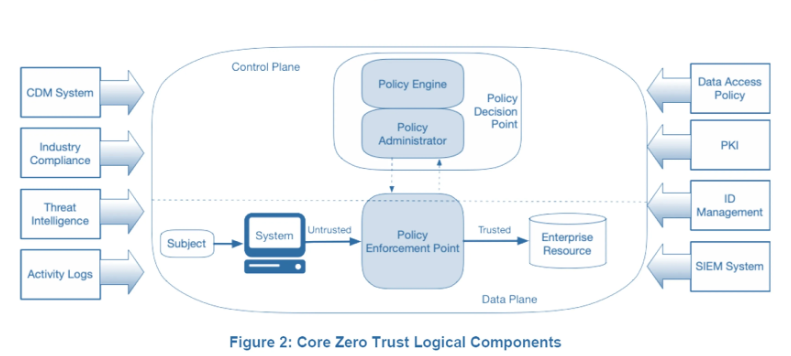
\includegraphics[width=0.65\linewidth]{figures/ZT components.png}
    \caption{Logical components of the ZT\cite{stafford2020zero}}
    \label{fig:logicalcomp}
\end{figure}

\subsection{The ZT importance in 5G}
Given the numerous benefits that Zero Trust (ZT) brings in terms of enhanced security and the challenges associated with 5G networks, it seems like a promising approach to integrate ZT into the 5G architecture. The dynamic and distributed nature of 5G, coupled with its increasing complexity, makes traditional security models inadequate. Zero Trust's ability to provide continuous authentication, strict access controls, and robust threat mitigation aligns well with the evolving security needs of 5G, making it an ideal candidate to address these emerging challenges.




%% Threatmodeling
\section{Threat modelling and Risk Assessment}
In this section, we analyze the security of 5G networks with a particular focus on the critical interfaces that interconnect Network Functions (NFs). These interfaces play a vital role in the operation of the 5G system (5GS) and are crucial to prioritize as they carry sensitive signaling information, user data, and other confidential details that are potential targets for attackers.

Rather than providing a broad overview of 5G security, this analysis
emphasizes interface-level security, which is essential for identifying vulnerabilities and risks that span multiple architectural implementations. These critical interfaces are integral to various 5G RAN architectures, including Open RAN, Virtualized RAN, Cloud RAN, and the 5G Core (5GC). Through this detailed assessment, we aim to identify vulnerabilities and risks that could compromise the security and performance of the 5G network.


\subsection{Threat Analysis Methodology}
The interface-level security assessment covers the following aspects:
\begin{itemize}
    \item \textbf{Identification of Critical Interfaces:} Recognizing interfaces that handle sensitive signaling information, user data, and confidential information.
    \item \textbf{Threat modelling: }Assessing potential threats to these interfaces Using the STRIDE threat model.
    \item \textbf{Risk Mitigation}: Discussing security measures that protect these interfaces, such as encryption, authentication, and continuous monitoring.
\end{itemize}

\subsection{Security Goals}
To secure the 5GS, the 3GPP outlines five primary security goals:\cite{mahyoub2024security}
\begin{enumerate}
    \item \textbf{Confidentiality:} Ensures only authorized users can access sensitive information. 
    \item \textbf{Integrity:} Protects data from unauthorized modification during transmission.
    \item \textbf{Authentication:} Verifies the identities of entities (e.g., NFs, UEs) before communication.
    \item \textbf{Replay Protection:} Prevents attackers from capturing and reusing packets to impersonate legitimate users.
    \item \textbf{Privacy:} Protects user-sensitive data, ensuring it is only used for its intended purposes.
    
\end{enumerate}

\section{Threat modelling of Critical interfaces}
\begin{figure}[H]
    \centering
    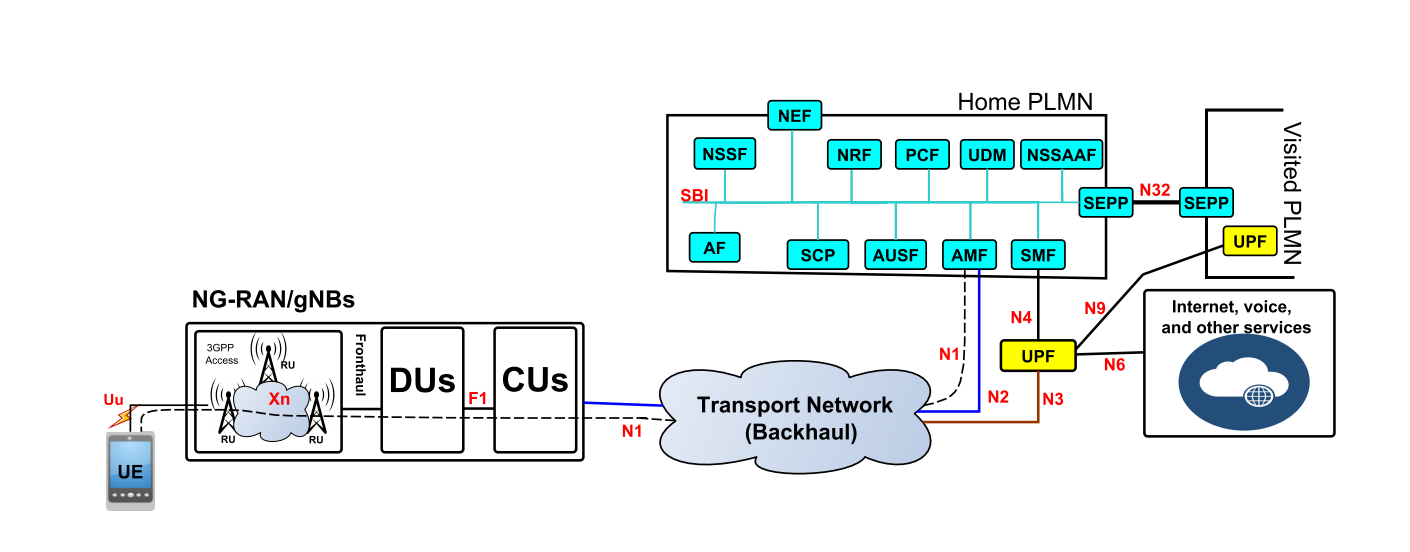
\includegraphics[width=1\textwidth]{figures/interfaces.png}
    \caption{5G Architecture with Critical interfaces in Red }\cite{mahyoub2024security}
\end{figure}

\subsection{N1 interface}

The N1 interface is critical to the functionality of the 5GS, enabling user session management, mobility management, and network access control. It facilitates NAS (Non-Access Stratum) signaling between the UE and the AMF, including authentication, authorization, data connection management, and mobility-related information exchange.

\subsubsection{Vulnerability and Threats}
Several attacks can exploit the N1 interface if proper security measures are not implemented. Key threats are presented below.A summary of all threats are presented in Table~\ref{tab:threats_summary}.
\begin{itemize}
    \item \textbf{AMF Impersonation:} If an attacker pretends to be the legitimate AMF and successfully serves the UE, false UE authentication could occur, revealing the SUPI and compromising authentication and authorization activities.\cite{mahyoub2024security}
    \item \textbf{IMSI Catcher:} Although mitigated in standalone 5G deployments, this attack is still possible in non-standalone deployments, especially if SUPI concealing isn't correctly implemented.
    \item \textbf{Request Flooding:} A malicious gNodeB or rogue UE can exhaust UE resources by sending\cite{mahyoub2024security} multiple identifier request messages, forcing the UE to respond with its SUCI each time.
    \item \textbf{NAS Protocol Vulnerabilities:} The NAS protocol supports critical signaling functions such as UE mobility, authentication, identification, and session management. If the authentication procedure fails during initial registration from a rogue UE, an attacker can exploit this to perform DoS attacks, MiTM attacks, or leak subscriber identities.
    \item \textbf{Bidding Down Attacks:} These attacks can force the system to use weaker security algorithms, increasing vulnerability.\cite{mahyoub2024security}
\end{itemize}

\subsubsection{Security Recommendations}
To mitigate these vulnerabilities, the following security measures are recommended by 3GPP, ETSI, ITU, and GSMA. \cite{mahyoub2024security}
\begin{enumerate}
    \item \textbf{Confidentiality:} Null ciphering algorithm (NEA0), 128-bit SNOW 3G-based algorithm (128-NEA1), and 128-bit AES-based algorithm (NEA2). 128-bit ZUC-based algorithm (128-NEA3), where regulations permit.
    \item \textbf{Integrity:} NIA0, 128-NIA1, and 128-NIA2 for message authentication code integrity protection.
    \item \textbf{Authentication: }EAP-TLS and improved EAP-AKA’ (using HMAC-SHA-256) to prevent bidding down attacks. EAP-TLS 1.3 for enhanced security and reduced latency.
    \item \textbf{Replay Protection:} Receivers should accept each NAS/PDCP COUNT value only once and periodically update KSEAF keys.
    \item \textbf{Privacy:} SUPI should not be transmitted in plain text, except for routing information and unauthenticated emergency calls. SUCI (Subscription Concealed Identity) and 5G-GUTI (Globally Unique Temporary Identity) should be used instead.
\end{enumerate}

\subsection{Xn, F1 and N2 interfaces}
\textbf{Xn Interface:} The Xn interface facilitates handovers between source and target gNB/NG-eNB during mobility. It transfers sensitive information such as UE security capabilities, ciphering algorithms, and integrity algorithms, which require robust protection\cite{mahyoub2024security}.\\

\noindent \textbf{F1 Interface: }The F1 interface connects gNB-DUs and gNB-CUs within the 5G RAN. As it carries both signaling and user data, it is a critical target for potential attacks\cite{mahyoub2024security}.\\

\noindent \textbf{N2 Interface: } The N2 interface links the RAN and AMF, facilitating NAS message exchange between 3GPP and non-3GPP access networks to the 5GC. Control Plane (CP) data on the N2 interface is protected with integrity, confidentiality, replay protection, and mutual authentication mechanisms between the NG-RAN and AMF.

\subsubsection{Vulnerability and Threats}
The table below presents the threats to the interfaces.


\begin{table}[H]
    \centering
    \caption{Threats to Xn, F1, and N2 Interfaces \cite{mahyoub2024security}}
    \renewcommand{\arraystretch}{1.2} 
    \setlength{\tabcolsep}{5pt} 
    \begin{tabularx}{\textwidth}{|l|l|X|X|c|c|c|c|c|c|}
    \hline
    \textbf{Interface} & \textbf{End Points} & \textbf{Vulnerability} & \textbf{Assets} & \textbf{S} & \textbf{T} & \textbf{R} & \textbf{I} & \textbf{D} & \textbf{E} \\ 
    \hline
    \multirow{4}{*}{Xn} 
        & \multirow{4}{*}{gNB $\leftrightarrow$ gNB} 
        & CP integrity protection & CP data, processing capacity & $\bullet$ &  &  & $\bullet$ &  &  \\ \cline{3-10}
        & & UP confidentiality at gNB & UP data & $\bullet$ &  &  & $\bullet$ &  &  \\ \cline{3-10}
        & & Bidding down on Xn-handover & Mobility management data, processing capacity & $\bullet$ & $\bullet$ &  &  &  &  \\ \cline{3-10}
        & & CP confidentiality protection & User account data and credentials, mobility management data &  & $\bullet$ &  & $\bullet$ &  &  \\ \hline
    
    \multirow{3}{*}{F1} 
        & \multirow{3}{*}{gNB-DU $\leftrightarrow$ gNB-CU} 
        & Malicious CP/replay CP & User credentials, RAN resources & $\bullet$ & $\bullet$ &  &  &  &  \\ \cline{3-10}
        & & Fake UP/replay UP & User credentials, RAN resources & $\bullet$ & $\bullet$ &  &  &  &  \\ \cline{3-10}
        & & Eavesdropping & User credentials, RAN resources & $\bullet$ &  &  & $\bullet$ &  &  \\ \hline
    
    \multirow{8}{*}{N2} 
        & \multirow{8}{*}{gNB $\leftrightarrow$ AMF} 
        & False base-station attack & gNBs and AMFs & $\bullet$ &  &  &  &  &  \\ \cline{3-10}
        & & De-synchronization attack & User subscription profile data, gNBs & $\bullet$ & $\bullet$ &  &  &  &  \\ \cline{3-10}
        & & Authentication complexity & Subscriber data and application/network data & $\bullet$ &  & $\bullet$ &  &  &  \\ \cline{3-10}
        & & Jamming attack & Network services, business services, RAN & $\bullet$ & $\bullet$ &  &  & $\bullet$ &  \\ \cline{3-10}
        & & Replay attacks & User credentials and user account data & $\bullet$ & $\bullet$ &  &  &  &  \\ \cline{3-10}
        & & Improper ciphering & System resources & $\bullet$ & $\bullet$ &  & $\bullet$ &  &  \\ \cline{3-10}
        & & Bidding down on Xn-handover & User credentials and user account data & $\bullet$ & $\bullet$ &  &  &  &  \\ \cline{3-10}
        & & Lack of integrity protection and verification of user data & User credentials and user account data & $\bullet$ & $\bullet$ &  & $\bullet$ &  &  \\ \hline
    
    \end{tabularx}
\end{table}


\newpage
\subsubsection{Security Recommendations}
To mitigate threats on the Xn, F1, and N2 interfaces, 3GPP and ETSI recommend the following:
\begin{itemize}
    \item \textbf{Confidentiality, Integrity, and Replay Protection:} Use IPsec ESP for encryption, IKEv2 certificate-based authentication for mutual key exchange, and Datagram Transport Layer Security (DTLS) for both control and user plane interfaces \cite{mahyoub2024security}.
    \item \textbf{Authentication:} DTLS is the recommended mechanism for authentication.
    \item \textbf{Privacy:} no specific recommendations identified \cite{mahyoub2024security}.
\end{itemize}
    

\subsection{N3, N4 and SBI Interfaces}
\noindent\textbf{N3 Interface:} The N3 interface connects the RAN to the UPF, requiring confidentiality, integrity, and replay protection. It carries user plane data from the 5G-AN to the UPF and facilitates bearer connections and mobility management by tracking user devices' movements\cite{mahyoub2024security}.\\

\noindent\textbf{N4 Interface:} The N4 interface links the SMF with the UPF, handling PDU session management, traffic steering, and reporting PDU events to the SMF. It also transmits lawful intercept targets and packet filtering templates, necessitating robust security measures due to the critical information it transports.\\

\noindent\textbf{SBI Interface:} The SBI connects the control plane's NFs in the 5GC. Security measures for the SBI depend on whether it is considered a trusted interface, with operators deciding on the implementation of security mechanisms.

\subsubsection{Vulnerability and Threats}
The table below presents the threats to the interfaces.


\begin{table}[H]
    \centering
    \caption{Threats to N3, N4, and SBI Interfaces \cite{mahyoub2024security}}
    \renewcommand{\arraystretch}{1.2} 
    \setlength{\tabcolsep}{5pt} 
    \begin{tabularx}{\textwidth}{|l|l|X|X|c|c|c|c|c|c|}
    \hline
    \textbf{Interface} & \textbf{End Points} & \textbf{Vulnerability} & \textbf{Assets} & \textbf{S} & \textbf{T} & \textbf{R} & \textbf{I} & \textbf{D} & \textbf{E} \\ 
    \hline
    \multirow{4}{*}{N3} 
        & \multirow{4}{*}{gNB $\leftrightarrow$ UPF} 
        & Misconfigured routing table & UEs & $\bullet$ &  &  &  &  &  \\ \cline{3-10}
        & & Flooding & System resources (UPF) & $\bullet$ & $\bullet$ &  &  &  &  \\ \cline{3-10}
        & & TEID uniqueness failure & UP and billing & $\bullet$ &  &  & $\bullet$ &  &  \\ \cline{3-10}
        & & MiTM attack & UE and 5G-SN location information, system resources & $\bullet$ &  & $\bullet$ & $\bullet$ &  &  \\ \hline
    
    \multirow{4}{*}{N4} 
        & \multirow{4}{*}{SMF $\leftrightarrow$ UPF} 
        & Data redirection & Network services, system resources & $\bullet$ & $\bullet$ &  &  &  &  \\ \cline{3-10}
        & & Flooding of fake PDU session creation request & System resources & $\bullet$ & $\bullet$ &  &  &  &  \\ \cline{3-10}
        & & Weak protection for signaling data & Session-related data &  & $\bullet$ &  & $\bullet$ &  &  \\ \cline{3-10}
        & & Session deletion/modification request & System resources & $\bullet$ & $\bullet$ &  &  &  &  \\ \hline
    
    \multirow{4}{*}{SBI} 
        & \multirow{4}{*}{NF $\leftrightarrow$ NF} 
        & JSON parser exploits & OS, NF file, user data and credentials, system resources, log data & $\bullet$ & $\bullet$ &  &  &  &  \\ \cline{3-10}
        & & JSON parser not robust & NF API, NF application, system resources &  & $\bullet$ &  & $\bullet$ &  &  \\ \cline{3-10}
        & & Rogue container & Other NF, the host, services & $\bullet$ &  & $\bullet$ & $\bullet$ &  &  \\ \cline{3-10}
        & & Flawed validation of credentials assertion & Core NFs resources, data, and services & $\bullet$ & $\bullet$ &  & $\bullet$ &  &  \\ \hline
    
    \end{tabularx}
\end{table}
    
\subsubsection{Security Recommendations}
    For confidentiality, integrity, replay protection, and authentication, 3GPP and ETSI recommend the following measures for the interfaces:
    \begin{itemize}
        \item \textbf{N4 Interface:} IPsec, TLS, HTTPS.
        \item \textbf{SBI :} TLS 1.2, IPsec, PKI, OAuth 2.0.
        \item \textbf{N3 Interface: } IPsec, ESP,IKEv2 certificates-based authentication \cite{mahyoub2024security}.
    \end{itemize}
    
\subsection{N9, N32 and N6 Interfaces}
    \noindent\textbf{N9 Interface: } The N9 interface connects two UPFs, carrying inter-PLMN UP traffic, including sensitive data that require protection from external exposure or alteration. This interface demands robust confidentiality and integrity protection, especially for signaling messages and security keys \cite{mahyoub2024security}.\\
    
    \noindent\textbf{N32 Interface: } The N32 interface links SEPPs in different PLMNs, used during roaming. It ensures integrity and confidentiality through protection policies, topology hiding, and message filtering at the application layer\cite{mahyoub2024security}.\\
    
    \noindent\textbf{N6 Interface:} The N6 interface conveys signaling and privacy-sensitive data to outside networks. It is vulnerable to attacks from connected Data Network Names (DNNs), making it crucial to secure this interface to mitigate external threats.
    

\subsubsection{Vulnerability and Threats}
    The table below presents the threats to the interfaces.
    
\begin{table}[H]
    \centering
    \caption{Threats to N9, N32, and N6 Interfaces \cite{mahyoub2024security}}
    \renewcommand{\arraystretch}{1.2} 
    \setlength{\tabcolsep}{5pt} 
    \begin{tabularx}{\textwidth}{|l|l|X|X|c|c|c|c|c|c|}
    \hline
    \textbf{Interface} & \textbf{End Points} & \textbf{Vulnerability} & \textbf{Assets} & \textbf{S} & \textbf{T} & \textbf{R} & \textbf{I} & \textbf{D} & \textbf{E} \\ 
    \hline
    \multirow{2}{*}{N9} 
        & \multirow{2}{*}{UPF $\leftrightarrow$ UPF} 
        & No protection for UP data & UP data & $\bullet$ & $\bullet$ &  &  &  &  \\ \cline{3-10}
        & & Invalid UP data forwarding & UP data &  &  & $\bullet$ &  &  & $\bullet$ \\ \hline
    
    \multirow{8}{*}{N32} 
        & \multirow{8}{*}{vSEPP $\leftrightarrow$ hSEPP} 
        & SEPP impersonation & UP and system resources & $\bullet$ &  & $\bullet$ &  &  &  \\ \cline{3-10}
        & & Incorrect handling for PLMN ID mismatch & Application layer security data, sufficient processing capacity & $\bullet$ & $\bullet$ &  &  &  &  \\ \cline{3-10}
        & & IPX impersonation & User data and system resources & $\bullet$ & $\bullet$ & $\bullet$ &  &  &  \\ \cline{3-10}
        & & Weak JWS algorithm & SEPP application & $\bullet$ &  &  & $\bullet$ &  &  \\ \cline{3-10}
        & & Exposure of confidential IEs in N32-f messages & SEPP application, service message transfer & $\bullet$ & $\bullet$ &  & $\bullet$ &  &  \\ \cline{3-10}
        & & Misplacement of encrypted IEs in JSON object by IPX & SEPP &  & $\bullet$ &  &  &  &  \\ \cline{3-10}
        & & Missing cryptographic material of peer SEPPs and IPX providers & SEPP &  & $\bullet$ &  & $\bullet$ &  &  \\ \cline{3-10}
        & & Policies mismatch & SEPP application, protection policies, system resources &  & $\bullet$ &  & $\bullet$ &  &  \\ \hline
    
    \multirow{1}{*}{N6} 
        & UPF $\leftrightarrow$ DN 
        & Malformed GTP-U messages & Processing capacity &  &  &  &  &  & $\bullet$ \\ \hline
    
    \end{tabularx}
\end{table}
 
\subsubsection{Security Recommendations}
    For the N32, N9, and N6 interfaces, 3GPP and ETSI recommend the following measures:\\
    
    \noindent\textbf{N32 Interface: }
    \begin{itemize}
        \item Use TLS between SEPPs in the absence of IPX entities.
        \item Use the PRINS protocol in the presence of IPX, which selectively encrypts necessary parts of transmitted messages.
        \item Implement JOSE as an application layer security mechanism for protecting roaming traffic \cite{mahyoub2024security}.
    \end{itemize}
    
    \noindent\textbf{N9 Interface:} Use IPsec for confidentiality, integrity, and replay protection.\\
    
    \noindent\textbf{N6 Interface:} Use IPsec for securing data transmission.
    
%% Chapter 4
\section{Literature review}
This section provides a synthesis of the articles reviewed on the security analysis of critical 5G interfaces and the integration of Zero Trust (ZT) principles in 5G networks.

% Begin the longtable environment
\begin{longtable}{|p{4cm}|p{12cm}|}
    \hline
    \textbf{Articles} & \textbf{Summary} \\ 
    \hline
    \endfirsthead % Header for all pages except the first
    \hline
    \textbf{Articles} & \textbf{Summary}  \\ 
    \hline
    \endhead % Footer for all pages
    \hline
    \endfoot
    \hline
    \endlastfoot
    
    \cite{mahyoub2024security} & This paper examines the security of key interfaces in the 5G system (5GS), emphasizing their role in interconnecting Network Functions (NFs) for data and service exchange. The study highlights the vulnerability of critical interfaces such as N1, N2, N3, SBI etc. due to their exposure to external networks and sensitive data handling. It categorizes threats using the STRIDE framework and analyzes security measures proposed by standardization bodies like 3GPP and ETSI.
    The paper also identifies gaps in existing security recommendations and suggests measures for confidentiality, integrity, authentication, replay protection, and privacy. It emphasizes the need for robust security mechanisms, including encryption protocols (e.g., IPsec, DTLS), key management strategies, and mutual authentication processes, to mitigate risks like spoofing, tampering, and information leakage.
    This work is notable for its interface-specific focus, offering a detailed analysis of vulnerabilities and threats, and providing insights for enhancing 5G interface security. \\
    \hline

    \cite{giambartolomei2024penetration} & This papermpresents a comprehensive security assessment of the 5G core from a web security perspective, focusing on vulnerabilities in service-based architectures and web technologies. Leveraging the STRIDE threat modeling framework, the authors identify key threats, including spoofing, tampering, information disclosure, and denial of service, in open-source 5G core implementations such as Open5GS, Free5GC, and OpenAirInterface.
    The study highlights specific vulnerabilities, such as SQL/NoSQL injections, brute force attacks, and directory traversal, emphasizing the importance of proper input sanitization, robust authentication mechanisms, and adherence to the principle of least privilege. \\
    \hline
    \cite{defenseindepth} & 
    \parbox[t]{12cm}{
    This article explores the principles of Zero Trust (ZT) applied to six components of 5G: endpoints, the air interface, radio base stations, Multi-Access Edge Computing (MEC), the 5G core network, and IoT applications. The goal is to propose an architecture and a defense-in-depth strategy aligned with ZT principles. The key proposals include:
    \begin{enumerate}
        \item \textbf{Endpoint/IoT Device Security:} Data encryption, PKI-based authentication for end devices and authentication of firmware and SIM cards for 5G network devices.
        \item \textbf{Air Interface Security:} Use of cyphering, integrity protection, and end-to-end encryption.  
        \item \textbf{Radio Base Station Security:} Certificates generating keys for each node, enhancing security over pre-shared keys and reducing key leakage.  
        \item \textbf{MEC Security:} Multiple controls based on the MEC architecture, with end-to-end encryption of control and user plane interfaces to ensure only authorized recipients can access and manipulate messages.  
        \item \textbf{5G Core Network Security:} Multiple controls to protect core functions from various attack surfaces, with each service-based architecture SBA function required to authenticate before accessing other functions.  
        \item \textbf{IoT Application or Internet Access Security:} Multiple controls to secure core exposure to external applications ensuring any application connecting to 5G functions is properly authenticated.  
    \end{enumerate}
    This analysis highlights security strategies that reinforce critical 5G components in accordance with ZT principles, aiming to limit unauthorized access and strengthen network integrity.
    } \\
    \hline

    \cite{ztran} &
    \parbox[t]{12cm}{
        This article explores integrating Zero Trust (ZT) methods into Open RAN (O-RAN), introducing the ZTRAN security framework comprising three microservices: authentication, intrusion detection, and secure slicing. O-RAN’s components (O-CU, O-DU, O-RU) present new challenges in user/network authentication, access control, data confidentiality, and resource integrity. 
        \begin{enumerate}
            \item ZTRAN Authentication xApp: Ensures secure user equipment (UE) identification through multi-factor authentication (MFA) and temporary random tokens for each UE, enforcing least privilege access.
            \item ZTRAN Intrusion Detection xApp: Continuously monitors data traffic for anomalies, using user behavior profiling to detect and flag suspicious activities, promptly sending alerts to mitigate threats.
            \item ZTRAN Secure Slicing xApp: Manages resource allocation by creating tailored slices for specific user requirements, with continuous monitoring to ensure optimal Quality of Service (QoS).
        \end{enumerate}
        This framework enhances security in O-RAN by integrating continuous authentication, anomaly detection, and precise resource control.
    }\\ 
    \hline

    \cite{izta} & 
    \parbox[t]{12cm}{
        The i-ZTA framework incorporates real-time monitoring, risk evaluation, and access decision-making using a dynamic trust algorithm (MED components). It aligns with the 3GPP 5G specification, leveraging the O-RAN architecture and machine learning for enhanced security. This paper is the first to propose an architectural concept for i-ZTA, setting a foundation for developing AI-driven security solutions in 5G/6G networks. In the i-ZTA architecture integrated into the O-RAN, each component plays a key role in managing the security of 5G/6G networks. 
        \begin{enumerate}
            \item Agent and Portal: The agent, a lightweight module on each network asset, collects data for risk assessment. The portal, intended for resource-constrained devices (IoT, sensors), manages access requests and supports federated learning with the agent.
            \item Intelligent Network Security State Analysis (INSSA): A graph neural network (GNN) is used to model the behavior of network nodes and assess access risks to resources. This model helps detect anomalies, including Denial of Service (DoS) attacks, and ensures compliance with security rules.
            \item Intelligent Policy Engine (IPE): The IPE makes the final decision on access authorization based on the agent's evaluation and the network's state. It uses a neural network to analyze historical activities and adjust security policies.
        \end{enumerate}
        This architecture relies on open interfaces in the O-RAN for data collection and real-time control, allowing for flexible and programmable security management. Integration with cloud platforms, MEC, and fog computing is planned for future research.
    } \\ 
    \hline

    \cite{secure5gandbeyond} & This article discusses the security challenges in 5G networks, which are built on a highly distributed, open service-based architecture, increasing the attack surface compared to traditional networks. The shift to cloud-native architectures, where monolithic applications are divided into microservices, has resulted in untrusted communication between these services, necessitating new cybersecurity measures. The article proposes integrating the Zero Trust model, which operates on the principle of "Never Trust, Always Verify," into access control systems. It emphasizes dynamically adjusting trust levels based on user behavior and recommendations. 
    - \textbf{TRBAC (Trust-Based Role-Based Access Control):} This model extends traditional RBAC by incorporating trust and risk elements, evaluating users not only by their roles but also by their behavior, trustworthiness, and associated risk. This dynamic approach helps secure assets by continually assessing user actions and adjusting privileges accordingly.  
    This dynamic approach helps secure assets by continually assessing user actions and adjusting privileges accordingly, addressing the evolving security needs of 5G cloud-native environments. \\ 
    \hline

    \cite{5gcsdp} & The following article addresses the 5G core network (5GC) architecture, based on Service-Based Architecture (SBA), which brings significant flexibility and innovation but also introduces security challenges due to the integration of various signaling protocols and virtualization complexities. The proposed solution is a 5GC-SDP architecture that combines Zero Trust principles with a Software-Defined Perimeter (SDP) approach, focusing on secure communication within the core network through Single Package Authorization (SPA). This ensures that only authenticated and authorized Network Functions (NF) can interact securely.  
    - SPA enhancement module: Using machine learning algorithms designed to counter SPA-related DoS attacks. 
    - 5GC-SDP architecture: This enhances core network security by reducing network exposure and implementing fine-grained access control, as demonstrated through tests against port scanning, DoS, and DDoS attacks.  
    The 5GC-SDP architecture effectively enhances core network security by reducing network exposure and implementing fine-grained access control. \\ 
    \hline
    
\end{longtable}

\section{Results and Discussions}
    The various articles reviewed have provided valuable insights into how Zero Trust (ZT) can be leveraged to enhance the security of 5G networks. These studies reveal a clear trend toward implementing ZT at the component level, allowing for a security model that operates independently from the core 5G components, whether in the Radio Access Network (RAN) or the Core Network.

    While these approaches demonstrate significant progress, they also highlight that the issue of achieving a truly comprehensive ZT framework for the entire 5G system remains unresolved. The goal of implementing Zero Trust across the entire network infrastructure is still a work in progress, as the current solutions address specific components or functions rather than securing the entire ecosystem.

    Furthermore, ZT is often applied by layering additional security measures onto existing network functions, rather than fundamentally altering their operation. This approach introduces new technologies and components without disrupting the core functionality of these systems. While this ensures minimal operational disruption, it also suggests that ZT is being added incrementally, and not yet fully integrated at the system-wide level.

    A key limitation in the implementation of Zero Trust is the interdependence and interoperability of the various solutions. While multiple technologies and approaches exist, the challenge lies in aligning them seamlessly to create a cohesive and unified ZT model across the entire 5G infrastructure. The heterogeneity of the technologies, including various vendors, network architectures, and legacy systems, creates significant barriers to achieving full interoperability. To realize a comprehensive Zero Trust implementation, it is crucial to address these challenges by ensuring that the diverse technologies can be integrated and aligned to work together effectively.

\subsection{Research Gap}
    While there's growing interest in ZTA and 5G security, a focused analysis on applying ZTA principles specifically to 5G critical interfaces appears to be relatively unexplored in existing literature. Hence there is a need to bridge this gap in future research.

\section{Conclusion}
    The objective of this work was to assess the current state of efforts surrounding the implementation of Zero Trust (ZT) within 5G networks. Our analysis highlighted a growing interest in leveraging ZT principles, as evidenced by an increasing number of studies focusing on this approach due to its ability to address various security challenges. However, these studies primarily target specific components of the system rather than providing security for the entire 5G ecosystem. This limitation often stems from a "trade-off" between achieving comprehensive security and maintaining operational efficiency.  

    Additionally, our research involved conducting a threat modeling exercise for the interfaces connecting the various Network Functions (NFs). This analysis revealed a significant gap: while security measures have been applied to critical interfaces, there is no existing literature or research specifically addressing the implementation of Zero Trust (ZT) on these interfaces. This finding opens up a new avenue for research, emphasizing the need for holistic security strategies that extend beyond individual components to secure the entire system.
\bibliographystyle{plain} % You can choose other styles like IEEEtran, alpha, etc.
\bibliography{references}


%% Appendix
\appendix
\section{Appendix A}


\subsection{Components of a Zero Trust Architecture}
\begin{table}[H]

    \begin{tabularx}{\linewidth}{|p{4cm}|X|}
       
    \hline
        \textbf{Component} & \textbf{Function} \\ \hline
        Policy Engine (PE) & Responsible for real-time access decisions, evaluating access requests based on policies considering identity, device status, time, location, and continuous diagnostics and mitigation (CDM) data. \\ \hline
        Policy Administrator (PA) & Defines and manages access policies based on the decisions of the PE, instructing the PEP to allow or terminate sessions based on access approvals or revocations. \\ \hline
        Policy Enforcement Point (PEP) & Activates, monitors, and terminates connections between subjects and resources according to policies defined by the PA and decisions from the PE. \\ \hline
        Continuous Diagnostics and Mitigation System (CDM) & Collects and analyzes real-time data to identify and mitigate security threats, ensuring the system's health and compliance. \\ \hline
        Industry Compliance System & Ensures compliance with regulatory requirements and industry standards relevant to the enterprise. \\ \hline
        Threat Intelligence Feeds & Collects data from various sources to inform access decisions, including information on attacks, vulnerabilities, and software flaws. \\ \hline
        Network and System Activity Logs & Records active logs, network traffic, and resource access activities to provide real-time information on the security state of the system. \\ \hline
        Data Access Policies & Defines the rules and regulations governing access to enterprise resources, either dynamically generated by the PE or encoded via a management interface. \\ \hline
        Public Key Infrastructure (PKI) & Manages certificates for resources, subjects, services, and applications, ensuring secure authentication and communication. \\ \hline
        Identity Management System & Manages user accounts, roles, access properties, and assigned resources within the enterprise, ensuring accurate identity verification. \\ \hline
        Security Information and Event Management System (SIEM) & Gathers and analyzes security-related information to adjust policies and prevent potential attacks on the enterprise's assets. \\ \hline
    \end{tabularx}
    \caption{Key Components of a Zero Trust Architecture}
    \label{tab:componentszta} 
\end{table}

\subsection{Security focuses in 5G}
    With the growing sophistication and frequency of attacks, the integration of Zero Trust (ZT) into 5G has become essential. This involves strengthening network access security, implementing continuous monitoring to detect threats, and preventing attackers from moving laterally within the network.\\
    \begin{enumerate}
        \item \textbf{Network Access Security}: Focuses on user equipment (UE) authentication and secure network access, addressing threats to the physical/radio interface and aligning with TS 33.501.
        \item \textbf{Network Domain Security}: Ensures secure data exchange between network nodes, including advancements in SDN, NFV, and MEC.
        \item \textbf{User Domain Security}: Protects user devices, following NIST guidelines to address device security concerns.
        \item \textbf{Application Domain Security}: Secures communication between users and application providers, leveraging blockchain and post-quantum cryptography for 5G applications.
        \item \textbf{Service-Based Architecture (SBA) Security}: Introduces new features for secure communication between network functions, focusing on registration, discovery, and authorization.
        \item \textbf{Visibility and Configurability}: Informs users about active security features across devices, the core network, and Open-RAN.
\end{enumerate}

\subsection{Threats to the N1 Interface}
\begin{table}[H]
        \centering
        \caption{Threats to the N1 Interface \cite{mahyoub2024security}}
        \label{tab:threats_summary}
        
        \renewcommand{\arraystretch}{1.2} 
        \setlength{\tabcolsep}{5pt} 
        \begin{tabularx}{\textwidth}{|l|l|X|X|c|c|c|c|c|c|}
        \hline
        \textbf{Interface} & \textbf{End Points} & \textbf{Vulnerability} & \textbf{Assets} & \textbf{S} & \textbf{T} & \textbf{R} & \textbf{I} & \textbf{D} & \textbf{E} \\ 
        \hline
        \multirow{19}{*}{N1} 
           & \multirow{19}{*}{UE $\leftrightarrow$ AMF} & A bidding down of UE capabilities & UE radio capabilities & $\bullet$ &  &  & $\bullet$ &  &  \\ \cline{3-10}
           &                          & AMF impersonation & UE identity & $\bullet$ &  & $\bullet$ & $\bullet$ &  &  \\ \cline{3-10}
           &                          & Registration request flooding & System resources & $\bullet$ & $\bullet$ &  &  &  &  \\ \cline{3-10}
           &                          & Inaccurate SUCI de-concealment & System resources &  & $\bullet$ &  & $\bullet$ &  &  \\ \cline{3-10}
           &                          & NAS protocol-based attack & UE data & $\bullet$ & $\bullet$ &  & $\bullet$ &  &  \\ \cline{3-10}
           &                          & Reuse 5G-GUTI & Mobility management data & $\bullet$ &  & $\bullet$ & $\bullet$ &  &  \\ \cline{3-10}
           &                          & IMSI catcher & UE identity & $\bullet$ &  & $\bullet$ & $\bullet$ &  &  \\ \cline{3-10}
           &                          & IMEI visibility & Device and user identity & $\bullet$ &  & $\bullet$ & $\bullet$ &  &  \\ \cline{3-10}
           &                          & Incorrect implementation of UE security capacity handling & User accounts, data, and credentials & $\bullet$ & $\bullet$ & $\bullet$ & $\bullet$ &  &  \\ \cline{3-10}
           &                          & AMF re-allocation & User data and credentials & $\bullet$ & $\bullet$ &  & $\bullet$ &  &  \\ \cline{3-10}
           &                          & 5G-GUTI and IMEI correlation & User location & $\bullet$ &  & $\bullet$ & $\bullet$ &  &  \\ \cline{3-10}
           &                          & Logical gNB jamming & Service availability & $\bullet$ & $\bullet$ &  &  &  &  \\ \cline{3-10}
           &                          & Physical radio jamming & Service availability and system resources & $\bullet$ & $\bullet$ &  &  &  &  \\ \hline
        \end{tabularx}
\end{table}



\end{document}
